\documentclass[10pt,letterpaper]{article}
\usepackage[top=0.85in,left=2.75in,footskip=0.75in,marginparwidth=2in]{geometry}

% use Unicode characters - try changing the option if you run into troubles with special characters (e.g. umlauts)
\usepackage[utf8]{inputenc}

% clean citations
\usepackage{cite}

% hyperref makes references clicky. use \url{www.example.com} or \href{www.example.com}{description} to add a clicky url
\usepackage{nameref,hyperref}

% line numbers
\usepackage[right]{lineno}

% improves typesetting in LaTeX
\usepackage{microtype}
\DisableLigatures[f]{encoding = *, family = * }

% text layout - change as needed
%\raggedright
\setlength{\parindent}{0.5cm}
\textwidth 5.25in 
\textheight 8.75in

% Remove % for double line spacing
%\usepackage{setspace} 
%\doublespacing

% use adjustwidth environment to exceed text width (see examples in text)
\usepackage{changepage}

% adjust caption style
\usepackage[aboveskip=1pt,labelfont=bf,labelsep=period,singlelinecheck=off]{caption}

% remove brackets from references
\makeatletter
\renewcommand{\@biblabel}[1]{\quad#1.}
\makeatother

% headrule, footrule and page numbers
\usepackage{lastpage,fancyhdr,graphicx}
\usepackage{epstopdf}
\pagestyle{myheadings}
\pagestyle{fancy}
\fancyhf{}
\rfoot{\thepage/\pageref{LastPage}}
\renewcommand{\footrule}{\hrule height 2pt \vspace{2mm}}
\fancyheadoffset[L]{2.25in}
\fancyfootoffset[L]{2.25in}

% use \textcolor{color}{text} for colored text (e.g. highlight to-do areas)
\usepackage{color}

% define custom colors (this one is for figure captions)
\definecolor{Gray}{gray}{.25}

% this is required to include graphics
\usepackage{graphicx}

% use if you want to put caption to the side of the figure - see example in text
\usepackage{sidecap}

% use for have text wrap around figures
\usepackage{wrapfig}
\usepackage[pscoord]{eso-pic}
\usepackage[fulladjust]{marginnote}
\reversemarginpar

% document begins here
\begin{document}
\vspace*{0.35in}

% title goes here:
\begin{flushleft}
{\Large
\textbf\newline{WEBNG: A templating tool for weighted ensemble sampling of rule-based models}
}
\newline
% authors go here:
\\
Ali Sinan Saglam\textsuperscript{1},
James R. Faeder\textsuperscript{1,*}
\\
\bigskip
\textsuperscript{1}Department of Computational and Systems Biology, University of Pittsburgh, Pittsburgh, PA 15260 USA
\\
\bigskip
\textsuperscript{*}faeder@pitt.edu

\end{flushleft}

\section*{Abstract}
Time scales for biological processes span many orders of magnitude, forcing modelers to tackle coupled processes that have large time scale gaps. This results in rare events, which take longer to occur than the fastest processes in the model. Efficient generation of rare events has been a focus of modelers for a long time and multiple software packages implement various rare event sampling algorithms. However, these packages frequently require expertise to get started with, making it harder for researchers to start using them. WEBNG (short for Weighted Ensemble--BioNetGen) is an open source software framwework that bridges the open source software packages WESTPA, which implements the weighted ensemble method for sampling rare events, and BioNetGen, which facilitates the specification and simulation of biochemical reaction network models following a rule-based approach. WEBNG simplifies rare event sampling in simulations of rule-based models by taking a model specified in the BioNetGen language (BNGL) and generating a WESTPA simulation folder ready to simulate with default parameters selected to match model observables. WEBNG is written in Python with dependencies only on proven, open-source packages that are in active development, which makes WEBNG easy to install and maintain. Here, we describe the architecture and features of WEBNG and demonstrate its capabilities through application to a two-gene model of cell fate transitions.

% now start line numbers
\linenumbers

% the * after section prevents numbering
\section*{Introduction}
%% Needs some reworking %AS - attempted to explain it better
Biological molecules can undergo many transformations, including phosphorylation, binding, ubiquitination, etc. The multisite/multivalent nature of many molecular components of biological networks gives rise to combinatorial complexity in the number of individual species (complexes) and reactions that can occur in the reaction network governing system dynamics \cite{hlavacek_complexity_2003}. To simplify modeling such systems, rule-based modeling approaches were developed to avoid manually enumeration of the network \cite{kappa2018,faeder2009rule}. Rule-based models define rules that specify how species can interact, and these rules are the applied iteratively to generate the network \cite{blinov2006graph}. BioNetGen (BNG)\cite{blinov2004bionetgen,faeder2009rule,harris2016bionetgen} is an open-source rule-based modeling software package that allows for model construction in BioNetGen language (BNGL) and simulation of BNGL models.

Rare events in modeling are events that take a long time to occur compared to the time step used to simulate the model. Time scales on which biological processes happen span many orders of magnitude. Most biological models need to tackle coupled processes that happen at drastically different time scales\cite{peters2017reaction}, resulting in rare events. While in some models it is possible to simplify some of the faster processes to close the gap between time scales, in many models rare events are unavoidable because the fastest process in the system must be modeled for accuracy. 
Models with rare events can be computationally expensive to simulate because it takes many events to get a statistically robust estimate of any aspect of a biological process, which means the model has to be simulated for a long time in order to sample enough rare events.


Tackling this problem has been a focus of the computational modeling field and many rare event sampling methods have been developed \cite{wemain,tps1,tps2,ams,ffs}. One of these methods is called weighted ensemble path sampling method \cite{wemain}. Weighted ensemble path sampling works by organizing multiple parallel trajectories and 
resampling them at a fixed time interval to replicate trajectories that are making progress towards the rare event of interest and terminate trajectories that are not. Each trajectory is assigned a statistical weight that is tracked and updated during resampling in order to ensure that each trajectory that is generated has the correct statistical weight for computing system properties.

WESTPA is an open-source, scalable, and interoperable software package that applies the WE strategy \cite{westpa2022}. WESTPA has been successfully used to study multiple challenging biological processes \cite{weu1,weu2,weu3,weu4,weu5}
and is being actively developed. The fact that WE does not bias the kinetics of the model makes it easy to use with any model simulated with stochastic dynamics, including rule-based models. WESTPA has been designed with a general interface for stochastic simulation engines making it straightforward to couple with BioNetGen's \texttt{ssa} method, which implements an efficient version Gillespie's Direct Method \cite{gillespie1977exact} for stochastic simulation of reaction networks \cite{harris2016bionetgen}. 
%% JRF: Reader might naturally ask if this includes NFsim?

%% JRF: This paragraph seems pretty redundant now with the paragraphs starting at lines 107 and 111.
%%
%In biological modeling, researchers try to avoid working with models that contain rare events either because the computational cost is too high or because it is relatively easy to simplify the fastest processes and keep the timescale separation in a model relatively small, reducing computational cost. However, this does come at the cost of accuracy and not being able to understand how the kinetics of the fast processes in a model affect the slow ones. Rare event sampling methods can alleviate this issue, allowing researchers to tackle more detailed, challenging models that contain rare events.

To this end we have developed a tool called WEBNG (Weighted Ensemble--BioNetGen), which generates a WESTPA template for rare event simulation of a BNGL model. The user provides basic parameters for a WESTPA simulation along with a BNGL model to simulate, and the tool creates a WESTPA simulation folder that can then be run like any other WESTPA simulation. WEBNG is designed to tackle high dimensional WE simulations that are common for rule-based models and also provides several built-in analyses that are tailored to network-level simulations (as opposed to the molecular level simulations for which WESTPA was originally designed). WEBNG aims to lower the entry barrier for systems biology researchers to use the weighted ensemble method to explore models where rare events occur in an efficient way without having to learn details of the WESTPA interface that are needed for advanced applications.
%% worry about the computational cost.

\section*{Results}
%% TODO: Add subheadings. could be short descriptions for full sentences

\subsection*{WEBNG Architecture}
WEBNG comes with three subcommands that will set up the WESTPA simulation folder and analyze the resulting simulation in steps (Fig.~\ref{fig1}). The first subcommand, \texttt{template}, allows the researcher to point to the BNGL model file they want to simulate and this subcommand will generate a YAML file that is easy to read and modify and is populated with reasonable default values for package locations, WESTPA simulation parameters, and parameters for the built-in analyses, all of which can be modified by the user.

\begin{figure}[ht] %s state preferences regarding figure placement here
% use to correct figure counter if necessary
%\renewcommand{\thefigure}{1}
\centering
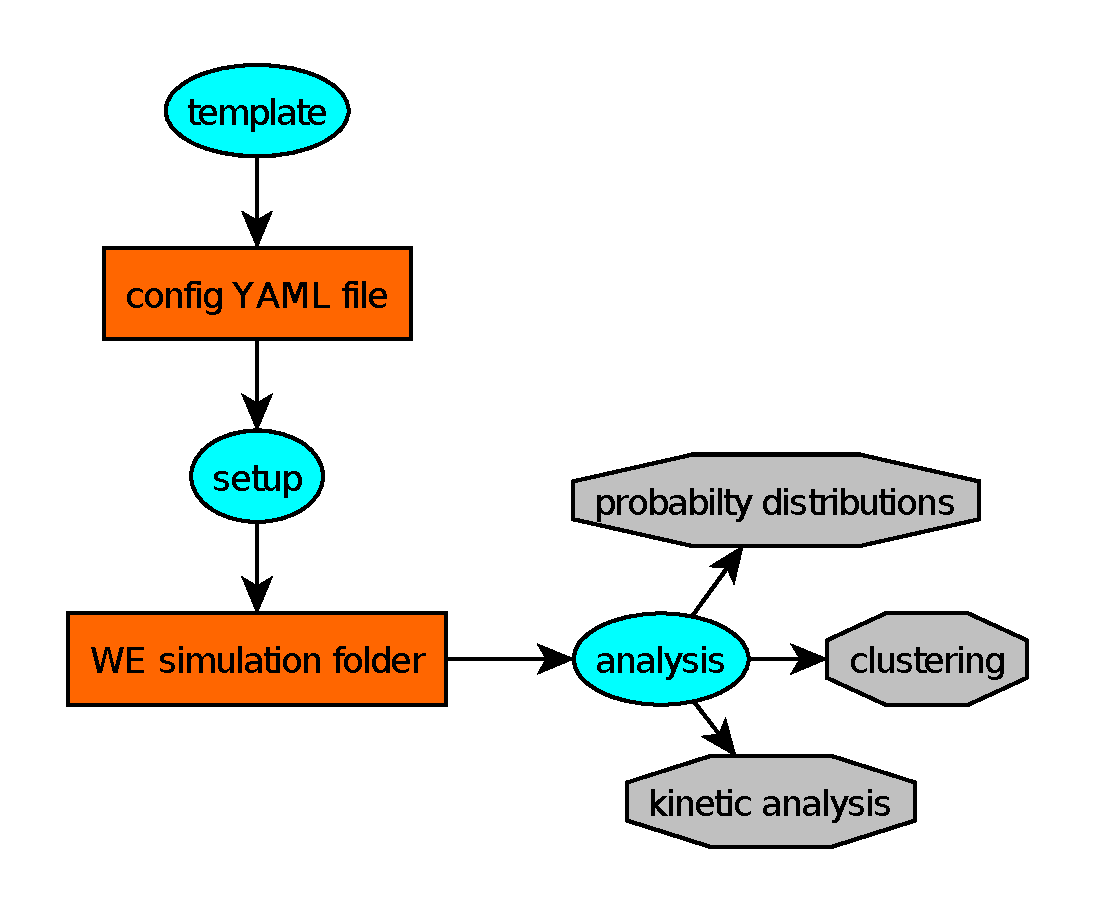
\includegraphics[width=2.5in]{fig1.pdf}
\caption{\color{Gray} \textbf{General workflow for WEBNG}. Elliptical nodes are WEBNG subcommands, rectangular nodes are files that are generated and passed between subcommands, hexagonal nodes are analysis results.}
\label{fig1} % \label works only AFTER \caption within figure environment
\end{figure}
%\clearpage

The next subcommand, \texttt{setup}, takes as a single argument the name of the YAML file generated in the previous step. This subcommand will use this information to generate the standard WESTPA simulation folder, which contains all of the files needed to carry out a simuluation using WESTPA. From this point the user can add more sophisticated options that are not currently supported by WEBNG prior to invoking WESTPA. For information on what options WEBNG currently supports, see the WEBNG documentation linked at the end of this paper. This workflow allows a new user to quickly start simulating their BNG model with reasonable defaults while also allowing an advanced WESTPA user to change simulation parameters and options freely. One important thing to note, by default WEBNG uses an adaptive Voronoi binning scheme\cite{voronoi} for the progress coordinates, which is a good starting point for high dimensional problems in the absence of further information. Binning strategies will be further discussed in the Results section. 

Once the simulation is run, the user can use the \texttt{analysis} subcommand, which also takes in the same YAML file generated in the \texttt{template} step. This subcommand will take in the parameters provided in the YAML file and run the enabled analyses on the simulation. The built-in analyses shown in Fig.~\ref{fig1} are \texttt{probability distributions}, \texttt{clustering}, and \texttt{kinetic analysis}. Here, we provide brief descriptions of each analysis method with detailed examples provided in the next section. 

There are two built-in probability distribution analyses, one that shows the joint probability distribution between every progress coordinate on a heatmap, and one that shows the evolution of the probability distributions of each progress coordinate. The joint probability distribution analysis is particularly useful to assess binning efficiency and simulation convergence. 

WEBNG allows for automated clustering using the Generalized Robust Perron Cluster Cluster Analysis (GPCCA+)\cite{pygpcca1} implemented in the PyGPCCA+ python library\cite{pygpcca2}. GPCCA+ is a generalized version of the clustering algorithm PCCA+\cite{PCCAp1,PCCAp2}, which is a clustering method based on the kinetics of a system. PCCA+ was originally designed to work on reversible systems under equilibrium, GPCCA+ extends this method to handle non-reversible systems as well. The user provides the number of clusters they want, and the GPCCA+ algorithm finds the ideal clustering of the bins in which transitions between clusters are minimized and transitions within clusters are maximized, maximizing the stability of each cluster while taking dominant cycles in the system into account. The resulting clustering can also be used in conjunction with WESTPA tools to calculate rate constants between clusters. Finally, WEBNG uses the clusters determined by GPCCA+ and the calculated transition matrices to make a GraphML file\cite{graphml}. This file can be opened in Gephi\cite{gephi} to visualize the clusters and transitions between them.

%% AS- First pass done for comments below

%% IDK if these are really commands per se or just general categories of methods. Anyway, I think the text below should be modified just to briefly describe what each is rather than referring to figure 2, which doesn't make much sense until you've seen the ExMISA model. 
% {\color{red}
% probability distributions of each progress coordinate over WE iterations (Fig2B), (2) 2D joint probability distributions of each progress coordinate against each other progress coordinate, (3) calculation of the transition matrix and PCCA+ clustering based on the transition matrix as well as calculation of rate constants between PCCA+ clusters 
% %% Note that rate constants are not shown in panel C. It could be useful to show a table of the transition rates to make explicit that these are computed and that both their means and stderrs are available (if true). 
% %% A more minor point is that PCCA+ appears without definition or reference, so the reader is just expected to know what this is? In general, it may be wortwhile to provide any details about what additional tools/methods are used for the analysis and visualization, especially ones that are specific to WEBNG. yEd could also be cited for instance. 
% (Fig2C) and (4) network graphs that visualize the calculated clusters and transitions between them (Fig2D). These analyses are complicated for a new user to implement since the user not only needs to know how to program but also needs to learn how WESTPA files are structured. WEBNG allows a new user to start analyzing the WESTPA simulation immediately; analyses 1 and 2 are useful for tracking simulation progress and analyses 3 and 4 identify important states in the progress coordinate space and calculate rate constants between them.}

\subsection*{WEBNG Installation}

WEBNG is distributed via the Python Package Index (PyPI), which simplifies installation to a single command from the command line. Installing WEBNG also installs PyBioNetGen (a Python package that comes with BioNetGen) and WESTPA. This not only allows the user to avoid having to install the other two packages separately but also enables the \texttt{template} command to automatically locate the other packages and provide their paths in the YAML configuration file.

%% Would be nice to show the execution/simulation step in here also
\subsection*{Application of WEBNG to a Gene Expression Model}

Tse et al.\ used weighted ensemble to run stochastic simulations of multiple gene regulatory network models, identify different phenotypes of the model, and estimate mean first passage times between those phenotypes. We used this study as a guide in designing of WEBNG with the aim to quickly set up simulations for the systems used in the paper and replicate the analyses in a streamlined fashion. Here, we have replicated the results of the exclusive mutual inhibition and self-activation (ExMISA) model shown in Fig.~\ref{fig2}. In this model, two genes, A and B, encode transcription factors that activate their own transcription and repress the transcription of the other gene. The model includes the creation and degradation of the transcription factors as well as binding and unbinding of these transcription factors to the regulatory regions of both genes. 

\begin{figure}[ht] %s state preferences regarding figure placement here
\centering
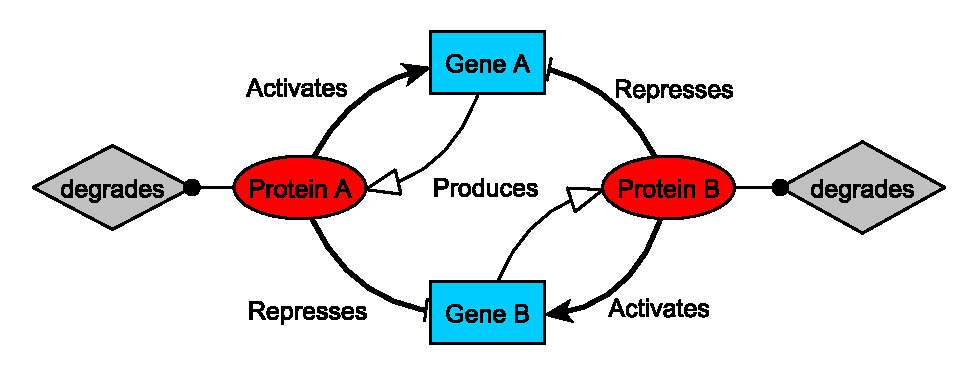
\includegraphics[width=\textwidth]{fig2.pdf}
\caption{\color{Gray} \textbf{Diagram of the genetic switch model ExMISA\cite{TseRead}}.}
\label{fig2} % \label works only AFTER \caption within figure environment
\end{figure}

%% JRF: I think we should walk the reader briefly through the workflow and in particular discuss the WE parameters that were chosen.

The analysis reveals four expected high probability regions (Fig.~\ref{fig3}(A)), one region where both proteins are low in count (lo/lo), one where both proteins are high in count (hi/hi) and two regions where one protein is low and the other is high in count (hi/lo and lo/hi). The automated clustering correctly identifies each cluster (Fig.~\ref{fig3}(B)) and automated network visualization can visualize each state and transitions between them (Fig.~\ref{fig3}(C)). Standard WESTPA tools can also be used to calculate the rate constants and therefore mean first passage times (MFPTs) between phenotypes identified from clustering (Fig.~\ref{fig3}(C)).

%% JRF: Should provide link to code that can regenerate these results

\begin{figure}[h!] %s state preferences regarding figure placement here
\centering
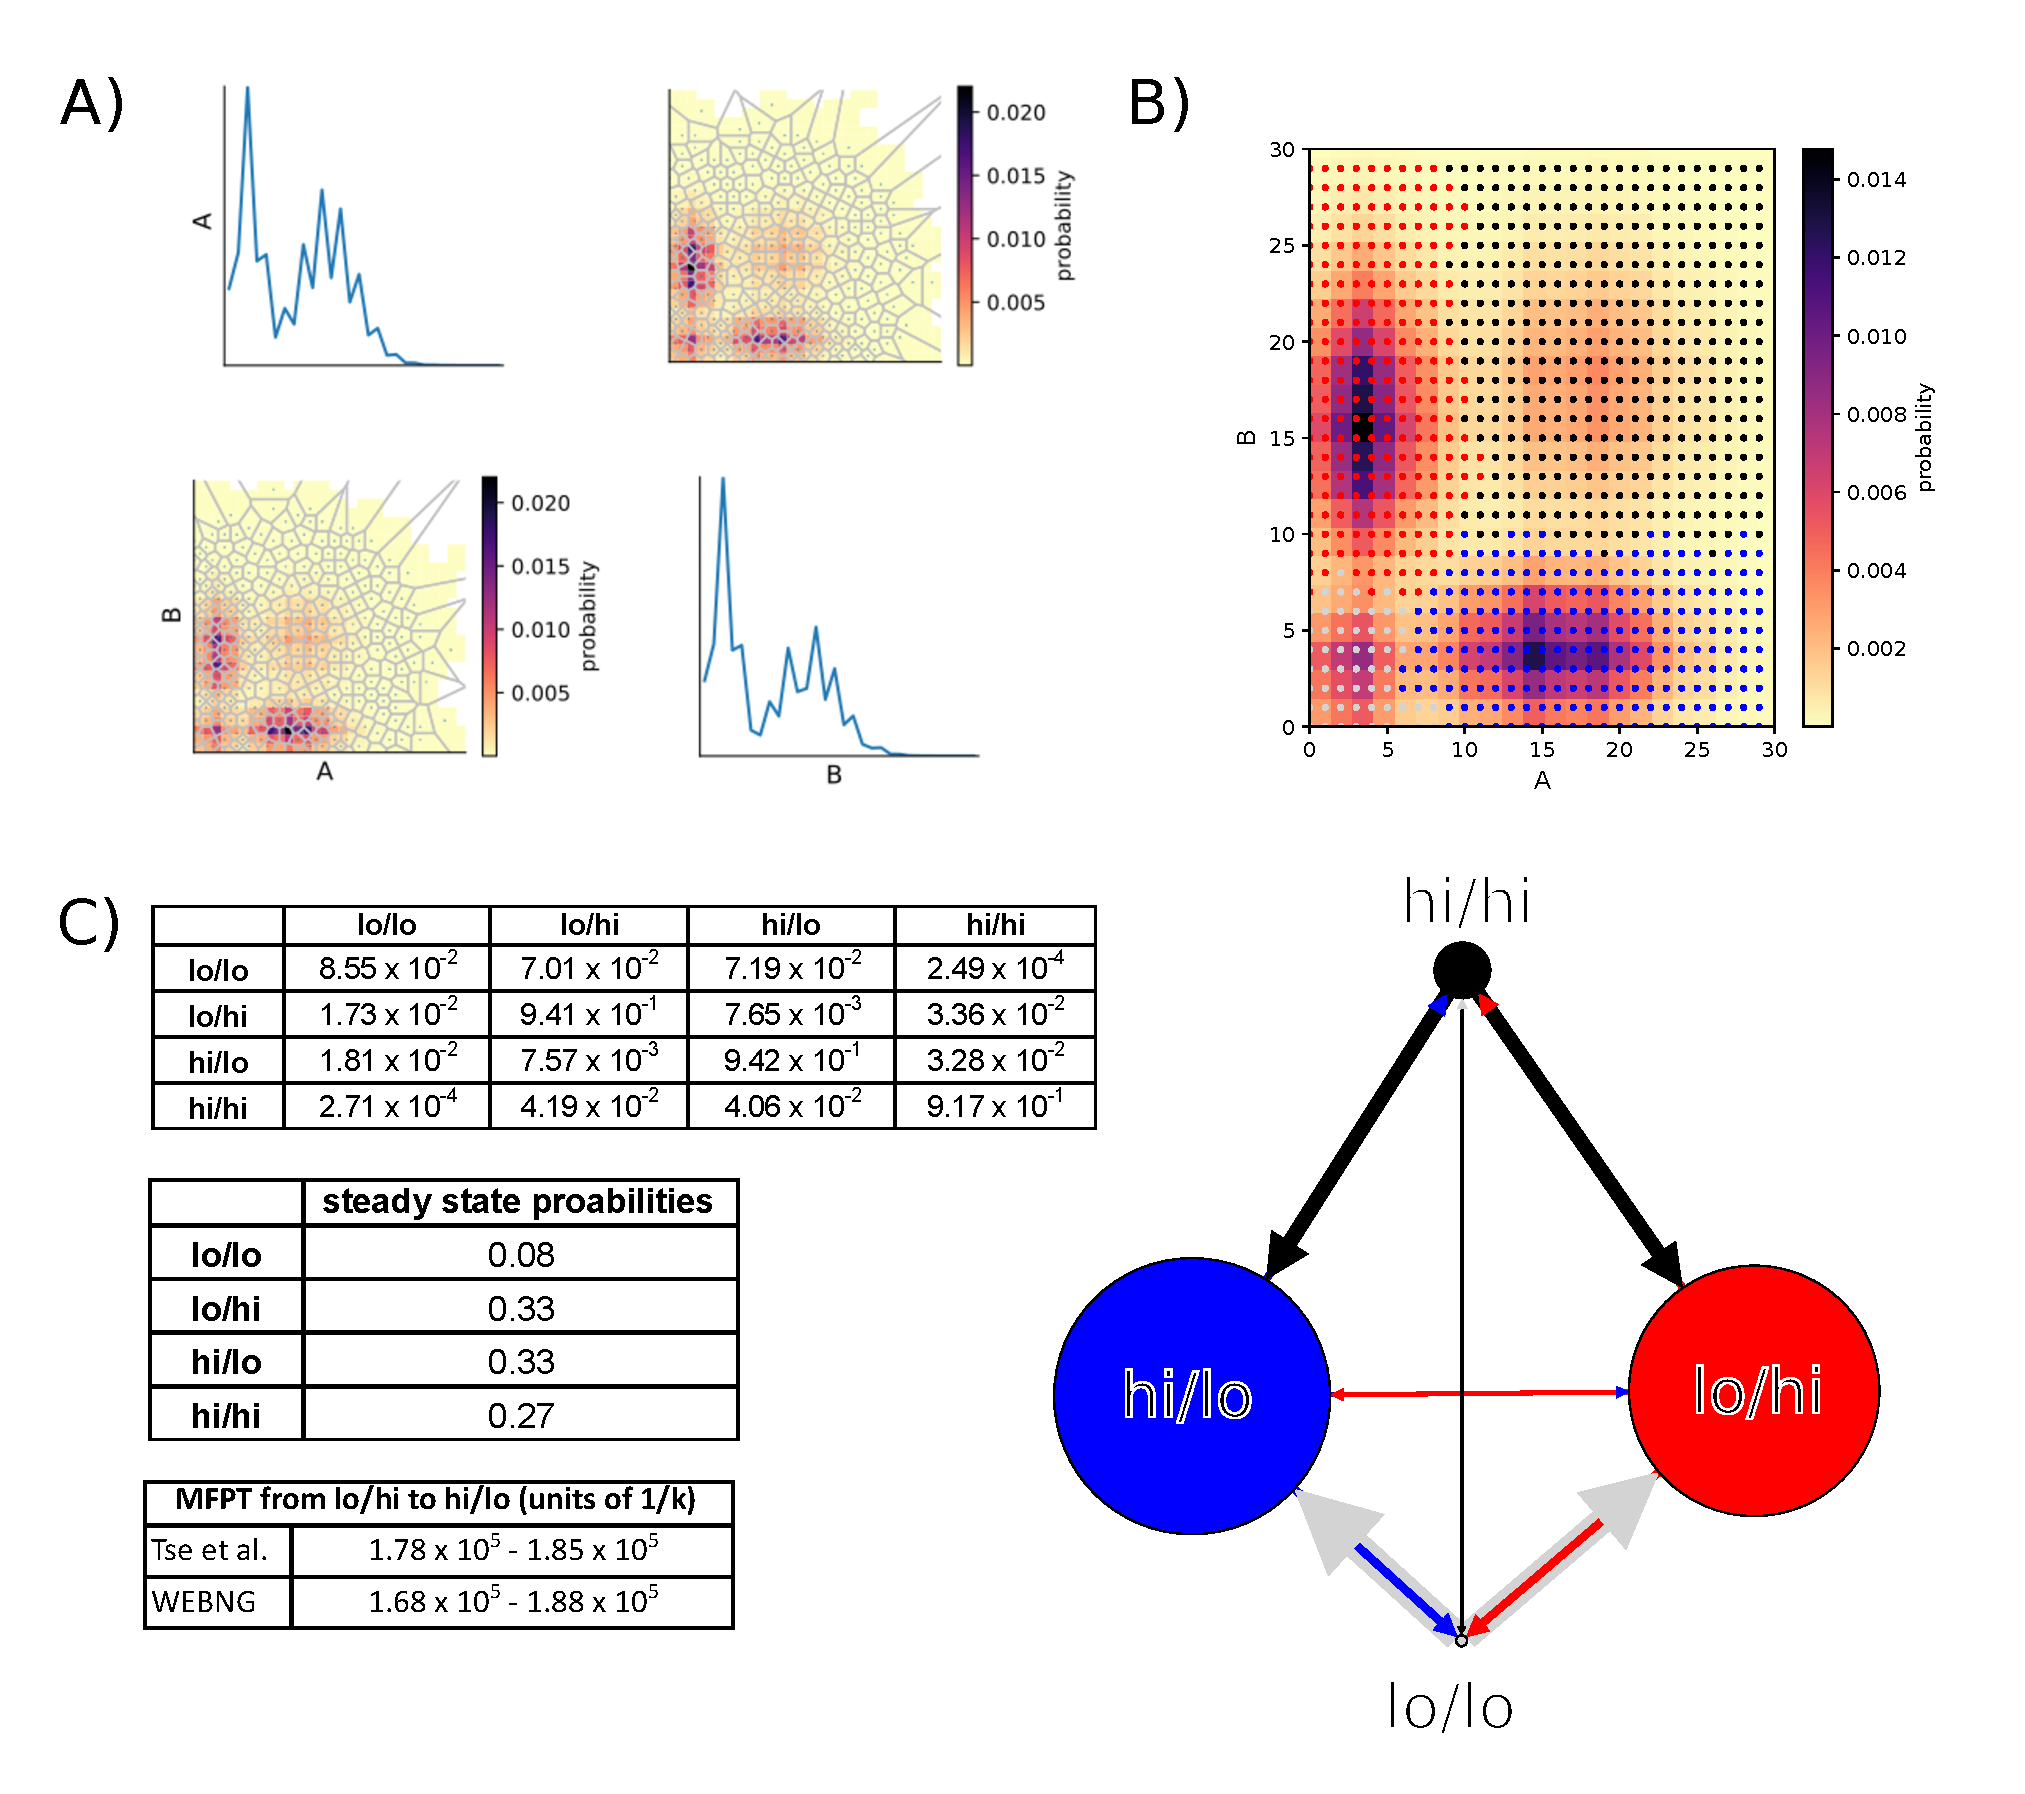
\includegraphics[width=\textwidth]{fig3.pdf}
\caption{\color{Gray} \textbf{Diagram of the genetic switch model ExMISA\cite{TseRead} and results of automated analyses on a WE simulation}. \textbf{A-C}, The WE simulation was run for 500 iterations (A) 2D heatmaps of joint probability distributions of protein A versus protein B counts. Lighter colors show less probable regions while darker colors show more probable regions. The probability distributions are estimated over the last 100 WE iterations. The grey lines indicate Voronoi bins used in adaptive binning. (B) Automated clustering correctly identifies each high probability phenotype. Clusters are represented by colored dots overlaid on top of a 2D heatmap of joint probability distribution of protein A counts versus protein B counts. Each colored dot represents one discrete possible state the model is in and each color represents a different cluster. (C) Transition probabilities between GPCCA+ generated clusters and steady state probabilities estimated from those transitions. MFPT is estimated using WESTPA tools and using definitions that match Tse et al.\ study. Network graph is automatically generated from the transition matrix and the steady state probabilities. Thicker edges mean higher probability transitions between clusters and node sizes scale with the probability of each phenotype in steady state. Each edge is colored by the state that they start from.}

%% AS-Addressed the coloring, more symmetric graph instead. 
%% This last point is a bit confusing, because the lo/lo state appears to be colored white (at least in panel (C) but the edges are gray in (D). I also wonder if it's possible to make this graph look more symmetric? Both the gray and black transition lines switch orientation between top and bottom, making it look like the transition rates are less symmetric than they actually are. 

%% JRF: In (C) you switched from using lo and hi to refer to states to 'l' and 'h'. As the figure stands, there is no panel (D). It's also not labeled as such in the caption.

\label{fig3} % \label works only AFTER \caption within figure environment
\end{figure}

%\clearpage

\section*{Discussion}
WEBNG is a simple templating tool that bridges two open software packages, WESTPA and BioNetGen, and lowers the barrier to entry to weighted ensemble rare event sampling of rule-based models. WESTPA, BNG and WEBNG are all well documented, which helps any potential researcher who wants to model processes that contain rare events using rule-based modeling by providing a simple starting point. BioNetGen also has the capability to take as input any model encoded using the Systems Biology Markup Language (SBML) standard \cite{keating2020sbml}. Using PyPI as the distribution point not only makes installation simple but also allows for all three software packages to be easily kept up-to-date and in sync. New analyses, higher simulation efficiency, and increased support for WESTPA parameters are currently in development for WEBNG.

Another advantage of a dedicated software package for templating these simulations is reproducibility. There are many studies where the model is implemented in a language-specific manner (including the Tse et al.\cite{TseRead}, in which the WE simulation is coded in MATLAB) 
%%(more example citations?) 
and contain hard-coded variables which makes reproducing results challenging even when the code is provided with the published paper. Dedicated software packages like WEBNG allow for the same simulation setup to be generated as long as the original model file is provided and results analyzed in a consistent manner to make results more reproducible.
%% Should cite recent Karr paper

More information on BioNetGen, WESTPA, and WEBNG can be found at the following links: \url{https://bionetgen.org/}, \url{https://westpa.github.io/westpa/}
and \url{https://webng.readthedocs.io/en/latest/}.

If you encounter any problems using WEBNG please report your problem under the GitHub issues page \url{https://github.com/ASinanSaglam/webng/issues}.

\section*{Acknowledgments}
We thank Elizabeth Read for helpful conversations about the two-gene model, Caleb Armstrong for proofreading and feedback on the manuscript, and Philipp Schlegel for the \LaTeX template, which can be found at \url{https://www.overleaf.com/latex/templates/arxiv-slash-biorxiv-template/phncddwqtxpc}. We also thank Dr.\ Berhard Reuter for helpful feedback regarding the appropriate description and citation of the clustering algorithms used by WEBNG. We gratefully acknowledge funding from NIH grants P41 GM103712 and R01 GM115805.

\nolinenumbers

%This is where your bibliography is generated. Make sure that your .bib file is actually called library.bib
\bibliography{library}

%This defines the bibliographies style. Search online for a list of available styles.
\bibliographystyle{plos2015}

\end{document}

